%File: formatting-instruction.tex
\documentclass{aamas2014}
%\documentclass[letterpaper]{article}

%\documentclass{aamas2013}
\usepackage{amsfonts}
\usepackage{amsmath}
\usepackage{algorithmicx}
\usepackage{algpseudocode}
\usepackage{algorithm}

%\fontsize{24}{6}
%\selectfont

%\usepackage{draftwatermark}
%\SetWatermarkScale{1}
%\SetWatermarkLightness{.9}
%\SetWatermarkAngle{-45}
%\SetWatermarkText{DRAFT DRAFT DRAFT DRAFT}


%\usepackage[usenames]{color}
\DeclareMathOperator*{\argmin}{argmin}

%\makeatletter
%\let\@copyrightspace\relax
%\makeatother

% if you are using PDF LaTex and you cannot find a way for producing
% letter, the following explicit settings may help

%\pdfpagewidth=8.5truein
%\pdfpageheight=11truein

\begin{document}

\AuthorsForCitationInfo{William Curran, Adrian Agogino, Kagan Tumer}

%\TitleForCitationInfo{Extending the Difference Reward to Multi-Objective Reinforcement Learning}

\title{Addressing Hard Constraints in the Air Traffic Problem through Partitioning and Difference Rewards}

\TitleForCitationInfo{Addressing Hard Constraints in the Air Traffic Problem through Partitioning and Difference Rewards}

%\titlenote{For use with aamas2011.cls}}

% AUTHORS

\numberofauthors{3}

\author{
Paper 605
%\alignauthor
%William Curran\\
%       \affaddr{Oregon State University}\\
%       \affaddr{Corvallis, Oregon}\\
%       \affaddr{curranw@onid.orst.edu}
%\alignauthor
%Adrian Agogino\\
%       \affaddr{NASA AMES Research Center}\\
%       \affaddr{Moffet Field, California}\\
%       \affaddr{adrian.k.agogino@nasa.gov}
%\alignauthor 
%Kagan Tumer\\
%       \affaddr{Oregon State University}\\
%       \affaddr{Corvallis, Oregon}\\
%       \affaddr{kagan.tumer@oregonstate.edu}
}

\maketitle


\begin{abstract}
Air traffic flow management over the U.S. airpsace is a difficult problem. Current management approaches lead to hundreds of thousands of hours of delay, costing billions of dollars annually. Routing decisions balancing delay with congestion contribute significantly to the propagation of delays throughout the US airspace. The task of managing delay may be seen as a multiagent congestion problem. 

In this problem there are many tightly coupled agents whose actions collectively impact the system, making it difficult for agents to learn how they individually affect the system. Reward shaping is effective at improving agent learning for soft constraint problems by reducing noise caused by interactions with other agents, so we extend those results to hard constraints that cannot be easily learned, and must be enforced algorithmically.

Our approach is based on the combination of three different methods to perform hard constraint optimization: a greedy scheduler, reward shaping and agent partitioning. Our results show that autonomous partitioning of the agents using system features leads to up to 450x speed over simple hard constraint enforcement, as well as up to a 37\% improvement in performance over a greedy scheduling solution, corresponding to hundreds of hours of delay saved in a single day.
\end{abstract}


\category{I.2.11}{Distributed Artificial Intelligence}{Intelligent Agents}
\terms{
Algorithms, 
%Management, 
%Measurement, 
%Documentation, 
Performance, 
%Design, 
%Economics, 
%Reliability%, 
Experimentation%, 
%Security, 
%Human Factors, 
%Standardization, 
%Languages, 
%Theory, 
%Legal Aspects, 
%Verification.
}
\keywords{Multiagent Reinforcement Learning, Air Traffic Control}






\section{Introduction}
A primary concern facing the aerospace industry today is the efficient, safe and reliable management of our ever-increasing air traffic. In 2011, weather, routing decisions and airport conditions caused 330,063 delays, accounting for 266,999 hours of delay \cite{faa05}. Many of these delays in the National Airspace System (NAS) are caused by en route, landing, or departing airspace congestion. The number of new flights being scheduled is faster than that of airports being built, making effective traffic control algorithms essential. We refer to the task of managing delay in the system by coordinating aircraft as the Air Traffic Flow Management Problem (ATFMP). 

Typical methods to alleviate delay in the ATFMP involve imposing ground delay on aircraft, changing the speed of en route aircraft, and changing separation between aircraft. Because the airspace has many connections from one airport to another, the congestion and associated delay can propagate throughout the system. Delays may be imposed to better coordinate aircraft and mitigate the propagation of congestion and the associated delay, but which aircraft should be delayed? The search space in such a problem is huge, as there are tens of thousands of flights every day within the United States \cite{faa05}.

Current approaches to the ATFMP include the use of binary integer programming \cite{Bertsimas}, evolutionary approaches \cite{Rios}, and multiagent reinforcement learning \cite{tumer-agogino_jaamas12}. The most recent complete overview of the ATFMP in practice is provided by Sridhar, Grabbe, and Mukherjee \cite{Sridhar}. These approaches reduce delay in the NAS, but either have not been expanded to an entire day of aircraft data or does not completely remove all congestion from the system. 

We propose an approach to solving the problem that blends multiagent coordination, reward shaping, hard constraints, and automated agent partitioning. Multiagent coordination turns the ATFMP into a distributed problem, thus decomposing it into smaller, more manageable problems. This coordination typically improves performance, but makes modeling interactions between agents much more difficult. When an agent takes an action with many other agents, the total reward of the system may not reflect the contribution of the single agent. 

Reward shaping is a field of multiagent reinforcement learning that focuses on the design of rewards, and has been shown to assist in multiagent coordination. The difference reward is a reward shaping technique that is helpful in discovering how much a single agent contributed to the overall system reward by calculating only the portion of the global reward to which a particular agent directly contributed. The combination of multiagent coordination and reward shaping give the ability to perform an intelligent guided search over tens of thousands of aircraft actions, while the hard constraint on congestion ensures a safe airspace.

In the ATFMP, multiagent coordination with reward shaping becomes a computationally intractable task, therefore we used automated agent partitioning to reduce the overhead associated with the hard constraint while computing rewards. Agents were only required to compute the reward relative to other agents within their partition, removing thousands of extra computations per learning step. We use automated agent partitioning and partitioned agents based on predicted agent interactions.

A high level view of the approach is as follows: First, we compute partitions of agents. These partitions are treated as reward independent of each other, and therefore need to only compute rewards relative to the other agents within their partition. We will use the term \textit{reward independent} to denote one partition of agents to have no impact on the reward of other partitions. Essentially, no matter what actions one partition of agents take, it will not affect the the action choice for any agent in another partition. We then perform multiagent reinforcement learning using the difference reward. Lastly, we introduce a greedy scheduler, removing all congestion from the system at the cost to delay. Again, combining the multiagent reinforcement learning with reward shaping and the greedy scheduler turns this into a computationally intractable task. However, with agent partitioning, rewards can be computed many times faster with minimal performance degradation.


\section{Background}
\label{sec:BACKGROUND}

To motivate our approach, we introduce previous work performed in the field of agent partitioning, a description and overview of the ATFMP, and describe the reward shaping technique used in this work.

\subsection{Agent Partitioning}

Previous work in agent partitioning has been to focus on what specifically to partition. Jordan and Jacobs \cite{716791} developed the Hierarchical Mixtures of Experts (HME) method to partition the state space directly, such that different agents can focus on specific regions of the state space. This method works well in non-linear supervised learning tasks. In this work all learning is unsupervised, so this technique cannot be used.

Partitioning actions so that each agent is responsible for a small number of actions is another approach used often. Sun and Pearson \cite{Sun98someexperiments} divided actions into two types, speed and turn, and each type was handled by a separate agent. This approach uses domain knowledge, and partitioning actions applies well in robotics, but not in domains where all actions need to be explored.

The last partitioning technique we describe is to partitioning system-level goals into smaller tasks. In the work by Dayan and Hinton \cite{Dayan93feudalreinforcement}, they accomplished goal partitioning through task allocation, where agents are organized in a hierarchy, where high-level agents assign goals to agents lower in the hierarchy on-line. In the work by Reddy and Tadepalli \cite{Reddy_learninggoal-decomposition}, the approach is more structured. In this work the partitioning of the goal is learned through externally provided examples. Overall, these approaches are under the assumption that the system-level goal can be subdivided, which is not always the case. 

In this work, we partition agents, essentially treating each partition of agents as an independent problem. Agents from one partition could potentially affect the environment of agents in another partition, but this work attempts to minimize the partition overlap. In a partitioning with complete reward independence, this work essentially treats the problem as a set of smaller and easier independent problems.


\subsection{Air Traffic Flow Management Problem}

The ATFMP addresses the congestion in the NAS by controlling ground delay, en route speed or changing separation between aircraft. The NAS is divided into many sectors, each with a restriction on the number of aircraft that may fly through it at a given time. This number is formulated by the FAA and is calculated from the number of air traffic controllers in the sector, the weather, and the geographic location. These sector capacities are known as en route capacities. Additionally, each airport in the NAS has an arrival and departure capacity that cannot be exceeded. Eliminating the congestion in the system while keeping the amount of delay each aircraft incurs small is the fundamental goal of ATFMP. 

Two popular approaches to simulating the ATFMP had been to develop Lagrangian models of each aircraft's dynamics, and to create aggregate models of the NAS \cite{Bertsimas:1998:ATF:767667.768027, Bilimoria, McNally, Mueller_analysisof}. In the Lagrangian model approaches, typically the trajectories of each aircraft are taken into account and either collision-avoidance or congestion-reduction is performed \cite{Bilimoria, McNally}. This is an accurate and fine-grained approach to the ATFMP, but also time-intensive and complex. On the other hand, aggregate models have been shown to simplify the NAS and therefore are a much simpler approach to the ATFMP. The aggregate models have been used in conjunction with linear programming to find solutions to air traffic flow \cite{Bertsimas:1998:ATF:767667.768027}, and linear algorithms to analyze departure, enroute and arrival delays \cite{Mueller_analysisof}.

In this work we chose to use an aggregate model of the NAS. By choosing to control the ground delay of each aircraft, rather than the enroute speed, and using historical data obtained from the FAA, we only need to count how many aircraft are within a particular sector at a particular time. Actions affect the simulation minimally, as an aircraft with imposed ground delay simply needs to shift its entire flight plan by the amount of ground delay, greatly speeding up simulation time.

Previous work in the ATFMP and scheduling had applied Integer Linear Programming \cite{Bertsimas}, evolutionary approaches \cite{Agogino:2009:EEM:1570256.1570258, Rios}, and multiagent approaches \cite{tumer-agogino_jaamas12,Curran:2013:AHC:2484920.2485183, 664154, Sislak:2008:AMA:1402744.1402755}. The ATFMP is a naturally distributed problem with complex interactions among all aircraft and airports. This renders predetermined centralized solutions suboptimal whenever there is any deviation from the expected air traffic flow. Therefore using a decentralized multiagent system is an ideal approach in such a domain.

There are three main issues to using Integer Linear Programming (ILP) that are removed using a multiagent approach; first, designing an ILP algorithm for a particular task is a difficult process, and it takes a lot of effort to adapt ILP to new problem variations that inevitably come up. Second, a formulation of ILP is complex even for simple problems. For real world implementations there is an enormous amount of subtle complexity that has to be included in the system, such as balancing the needs to airlines, air traffic controllers and passengers. These complexities can be added in a straightforward way in reward functions, but not in ILP. Third is computational complexity; ILP computation can grow exponentially with problem size. A carefully designed ILP can avoid this exponential increase within a certain range of parameters, but after a certain problem size, computing an ILP solution is infeasible, making it impracticable for the full ATFMP.

%Rather than treating congestion as a soft constraint, we approaches removed congestion completely from the system algorithmically through the use of a greedy scheduler. A high level view of this approach is as follows: First, they computed partitions of agents using a domain-based similarity metric of sector overlap and hierarchical agglomerative clustering. These partitions are treated as reward independent of each other, and therefore need to only compute rewards relative to the other agents within their partition. We will use the term \textit{reward independent} to denote one partition of agents to have no impact on the reward of other partitions. Essentially, no matter what actions one partition of agents take, it will not affect the the action choice for any agent in another partition. They then performed multiagent reinforcement learning using the difference reward. Lastly, they introduced a greedy scheduler, removing all congestion from the system. They found that combining the multiagent reinforcement learning with reward shaping and the greedy scheduler turns this into a computationally intractable task. They solved this problem with agent partitioning, showing that rewards can be computed many times faster with minimal performance degradation.

%\subsection{Heterogeneous bar problem}
%We introduce a modification to the bar problem where agents can go only a subset of nights.

%\subsection{Hierarchical reinforcement learning}
%Agent hierarchies are essentially what we are doing. We use hierarchical reinforcement learning to solve this problem. We decompose %the problem into a bunch of smaller problems. This is like Dietterich et. al.



\subsection{Reward Shaping}
Multiagent coordination is an important aspect of many domains, such as data routing \cite{tumer-wolpert_jair02}, air traffic control \cite{tumer-agogino_jaamas12}, Robocup soccer \cite{AAMAS12-agmon}, rover coordination \cite{5509316} and power plant operations \cite{Colby:2012:SFF:2343576.2343637}. A learning or evolutionary algorithm will often convert a once computationally intractable search problem into a feasible guided search. 

In learning algorithms reward design is important in keeping convergence time low while keeping performance high. In many multiagent coordination domains there is a difference between maximizing the system-level reward and maximizing a single agent's reward. If an agent always takes the locally-optimal action, it does not always maximize the system-level reward; this is known as the Tragedy of the Commons \cite{Hardin}.

The difference reward \cite{tumer-wolpert_jair02} is evaluated such that each agent's reward is related to the individual's contribution to team performance, therefore the signal-to-noise ratio is improved considerably. This leads to final better policies at an accelerated convergence rate. The difference reward is defined as:
%
\begin{equation}
D_i(z) = G(z) - G(z - z_i + c_i)\;,
\end{equation}
%
where \textit{z} is the system state, $z_i$ is the system state with agent $i$, and $c_i$ is a counterfactual replacing agent $i$. This counterfactual offsets the artificial impact of removing an agent from the system. For example, removing an aircraft from the system always artificially decreases the amount of congestion and delay, which would provide a poor reward if a counterfactual is not used.

The difference reward provides a compact encapsulation of the agent's impact on the system. It reduces the noise from other agents in the reward signal and has outperformed both system-level and local rewards in many congestion domains \cite{AAMAS12-agmon, Agogino:2012:ELS:2330163.2330306, Colby:2012:SFF:2343576.2343637, tumer-wolpert_jair02}. In many systems it is difficult or impossible to calculate the difference reward without resimulation, which can become prohibitively costly. If resimulation is fast, or the difference reward function is easily approximated, this reward function is a powerful tool for multiagent coordination.

\subsection{Constraint Optimization}
Typical learning algorithms use soft constraint optimization and attempt to minimize all objectives in the system. These are usually formulated as a multi-objective learning problem where agents receive a reward that is some combination of all objectives. Hard constraint optimization on the other hand can assist multiagent coordination by forcing a constraint to be satisfied, and attempting to optimize the rest of the reward. This approach simplifies a more complicated multi-objective coordination problem into a more simple single-objective problem.

One approach to constraint optimization is Distributed Constraint Optimization (DCOP) \cite{Junges:2008:EPD:1402298.1402308, Modi:2005:AAD:1120120.1120127}. DCOPs are well-suited for modeling multiagent coordination problems with many interactions between agents. We used multiagent reinforcement learning because of the large number of agents and intent to extend the scope of our experiments to include uncertainty in future work.

Greedy search algorithms, such as a greedy scheduler, can enforce hard constraints by forcing one of the objectives to 0 while sacrificing the other objectives. Previous approaches to the ATMFP use a greedy heuristic scheduler \cite{Rios} to enforce congestion constraints. The greedy scheduler checks to see if a plane's flight plan causes any sectors to become congested. If the plane causes congestion, it is delayed by one minute, and then the congestion is recalculated. This adds delay by completely removing congestion out of the system. The greedy scheduler is necessary in this domain to remove all congestion out of the system. This is a necessity of the problem: congestion in this domain means that there is not enough air traffic control personnel to handle the traffic.

Due to the heuristic nature of the scheduler, it is suboptimal and learning must be performed to improve performance. This solution requires a learning algorithm to first choose actions for the agents, then have those actions modified by the greedy scheduler, and finally reward the agents based upon the system after the greedy scheduler.

\section{ATFMP Approach}

Our approach to traffic flow management involved five main concepts: 
\begin{itemize}
\item Formulating a multiagent congestion problem by defining agents
\item Formulating the appropriate system reward function.
\item Reducing noise from the reward signal through reward shaping.
\item Enforcing hard constraints on congestion with the greedy scheduler.
\item Performing hard constraint optimization through agent partitioning
\end{itemize}

%A high-level view of the algorithm is as follows: First, during pre-processing we compute partitions of agents, these partitions are treated as being reward independent of each other, and during learning partitions need to only compute rewards relative to the other agents within their partition. We then perform multiagent reinforcement learning with the difference reward. Lastly, we introduce a greedy scheduler, which removed all congestion from the system at the cost of higher delays. Again, combining the multiagent reinforcement learning with the difference reward and the greedy scheduler turns this into a computationally intractable task, but with agent partitioning rewards can be computed hundreds or thousands of times faster.

\subsection{Agent Definition}
In this paper, agents were assigned to aircraft with cooperation enforced by airport terminals. Cooperation needs to be enforced because aircraft are naturally greedy. Aircraft are owned by different companies, and those companies are not interested in making sure aircraft from other companies arrive on time. This enforced cooperation assumption by aircraft terminals (or the government) is essential to remove greedy aircraft from the system.

Aircraft flight plans are from historical flight data from the FAA. Therefore, the only aspect of the environment we can change is the ground delay for each aircraft. Agents may select a certain amount of ground delay from 0 to 10 minutes (11 actions) in the beginning of every simulation. The FAA data has the sector location of each plane for every minute that plane was in service. Therefore, adding ground delay simply shifts a plane's flight plan over by that many minutes. The greedy scheduler then takes all plane flight plans, checks if the flight plans cause any congestion, and then further delays planes to eliminate congestion from the system.

%In this formulation, agents do not have the capability to change their action based upon the system once the simulation starts, therefore feedback can only be given once per simulation. Since agents are given no knowledge of the environment, they have no state. This simplifies the learning problem for each agent, as they only have eleven actions to sample from, but complicates the coordination. Agents must choose an action without prior knowledge of other agents choices, and must learn how the environment is changing, and simultaneously what action to take.

Agents learned using Action-Value Learning with a zero initialized value table. This is a stateless approach where agents map actions to values representing the quality of that action. 

%\subsection{Agent Learning}


%In single-agent systems, agents employing the exploration-exploitation strategies eventually come to an optimal solution \cite{Sutton98reinforcementlearning}. In multiagent systems the exploration of other agents become an issue. When an agent takes a greedy action, other agents can learn how that affected the environment, and modify their own greedy action. When an agent takes an exploratory action rather than a greedy action, other agents modify their greedy action based on how the environment changed with the exploratory actions. Agents learn to compensate for the exploratory actions in the system, so when exploration removed after some learning performance often decreases. This behavior is caused by exploratory noise \cite{holmes-aamas}.

%With so many agents in this system, exploratory noise causes a large problem. In the beginning of learning, having a large exploration is beneficial for the system. With 10\% of the agents taking random actions, we can find a good area of the reward space to explore. But near the end of learning, with most agents almost converged to a nearly optimal solution, 10\% of agents are taking random actions, causing over 3,500 agents to introduce noise into the learning of all other agents. To circumvent this problem, we need to have more agents performing greedy action selection as during each consecutive learning step. Therefore, $\epsilon$ would need to be lowered throughout learning to accomplish this. We approached this problem by reducing $\epsilon$ every n time steps by a constant amount (more sophisticated techniques such as the Boltzmann equation could be used, but only simple $\epsilon$ reduction was needed). The following equation was applied to $\epsilon$ at every time step:

%\begin{equation}
%\epsilon = \epsilon * c^{t * \Theta(t \mod n)}\;,
%\end{equation}
 
%where c is a constant value (typically .99), $t$ is the current time step and $\Theta(t \mod n)$ is a step function that equals 1 when $t \mod n$ is 0 and 0 otherwise, and $n$ is a value that varied depending on the number of learning steps. With more learning steps $n$ was higher, and in experiments with fewer learning steps $n$ was lower.

\subsection{Reward Structures}

The system-level reward we developed focuses on the cumulative delay ($\delta$) and congestion ($C$) throughout the system:
%
\begin{equation} \label{eq:Global}
G(z) = -(C(z)^w + \delta(z))\;,
\end{equation}
%
where $C(z)^w$ is the total congestion penalty to the power of $w$, and $\delta(z)$ is the cumulative system delay. The importance of congestion over delay is represented by the weight \textit{w}. Although minimizing delay is important, minimizing congestion is required for safety within the NAS. Therefore, minimizing delay must be performed simultaneously to minimizing congestion to zero, meaning the weight for congestion must be higher than delay.

The total delay is the sum of delays over all aircraft. This is a linear combination of the amount of ground delay and the amount of scheduler delay an agent incurred:
%
\begin{equation} \label{eq:Cumilative Delay}
\delta(z) = \displaystyle\sum\limits_{a \in A} (\delta_{g,a}(z) + \delta_{s,a}(z))\;,
\end{equation}
%
where $\delta_{g,a}(z)$ is the ground delay the aircraft incurred and $\delta_{s,a}(z)$ is the scheduler delay the aircraft incurred. 

The total congestion penalty is the sum of differences between sector capacity and the current sector congestion:
%
\begin{equation} \label{eq:Cumilative Congestion}
C(z) = \displaystyle\sum\limits_{s \in S} C_s(z)\;,
\end{equation}
%
where
%
\begin{equation}
C_s(z) = \displaystyle\sum\limits_{t \in T} \theta(C_{t,s} - S_s) (C_{t,s} - S_s)\;,
\end{equation}
%
where $S_s$ is the sector capacity of sector $s$ as defined by the FAA and $\theta$ is a step function that equals 1 if its argument is greater than 0, and 0 otherwise. In this way, agents are penalized when a sector exceeds its capacity.

Minimizing congestion involves intelligently adding ground delay to specific aircraft to obtain smallest amount of system congestion possible. In this problem, removing congestion from the system adds delay, and removing delay from the system could potentially add congestion, and as seen in Figure \ref{delayCongestionPower} this is not a direct mapping. Removing a little congestion from the system still requires the introduction of quite a bit of delay. Minimizing this cost to delay for every reduction in congestion is important to a stable solution.

With so many agents, tens of thousands of actions simultaneously impact the system, causing the reward for a specific agent to become noisy with the actions of other agents. An agent would have difficulty learning an optimal solution using such a noisy reward signal. A difference reward function reduces much of this noise, and is easily derived from the system-level reward:
%
\begin{equation}
D_i(z) = C(z-z_i + c_i)^w - C(z)^w + \delta(z-z_i + c_i) - \delta(z)\;,
\end{equation}
%
where \textit{$\delta(z-z_i + c_i)$} and \textit{$C(z-z_i + c_i)$} are the cumulative delay and congestion of all agents with agent $i$ replaced with counterfactual \textit{$c_i$}, with $w$ again being the importance of congestion over delay. 

We use a non-zero counterfactual for two reasons. One, an aircraft is removed from the system, the reward given to the agents is artificially increased. Furthermore, the aircraft are less likely to cause conflicts due to the easier scheduling problem. Two, we use a counterfactual where the agent does not delay at all, meaning that if not delaying produces a higher reward than delaying, this should be found quickly. We also take advantage of the fact that most airplanes do not need to be delayed. If the counterfactual is equal to the agent removed, the difference reward becomes zero and does not need to be calculated, thus speeding up reward calculations.

\subsection{Soft Constraint Application}

We want to convert a multi-objective problem into a single-objective problem. Multi-objective optimization adds a level of difficulty not essential to good performance in this domain. We can define a desirable solution in terms of a single value, in this case delay. 

We attempt to convert the multi-objective problem to a single-objective problem by increasing the exponential weight \textit{w} on the total congestion, as used in equation \ref{eq:Global} As \textit{w} increases, the delay impact on the system becomes negligible. Thus the agent will ignore the delay and only attempt to optimize congestion. This turned the multi-objective problem into a single-objective problem, but still kept sector congestion as a soft constraint.

Preliminary results, shown in Figure \ref{delayCongestionPower} indicate that this is an impractical solution. With a weight of one, the congestion and delay are equally optimized, leading to a balanced solution. When the weight on congestion increases to two or higher, the congestion converges to the same suboptimal point at different speeds. The agent will never evolve to an optimal policy that decreases congestion at the cost of delay, no matter how much emphasis is placed on congestion. Using exponential weights to convert this multi-objective problem to a single-objective problem does not work.

\begin{figure}[]
\centering
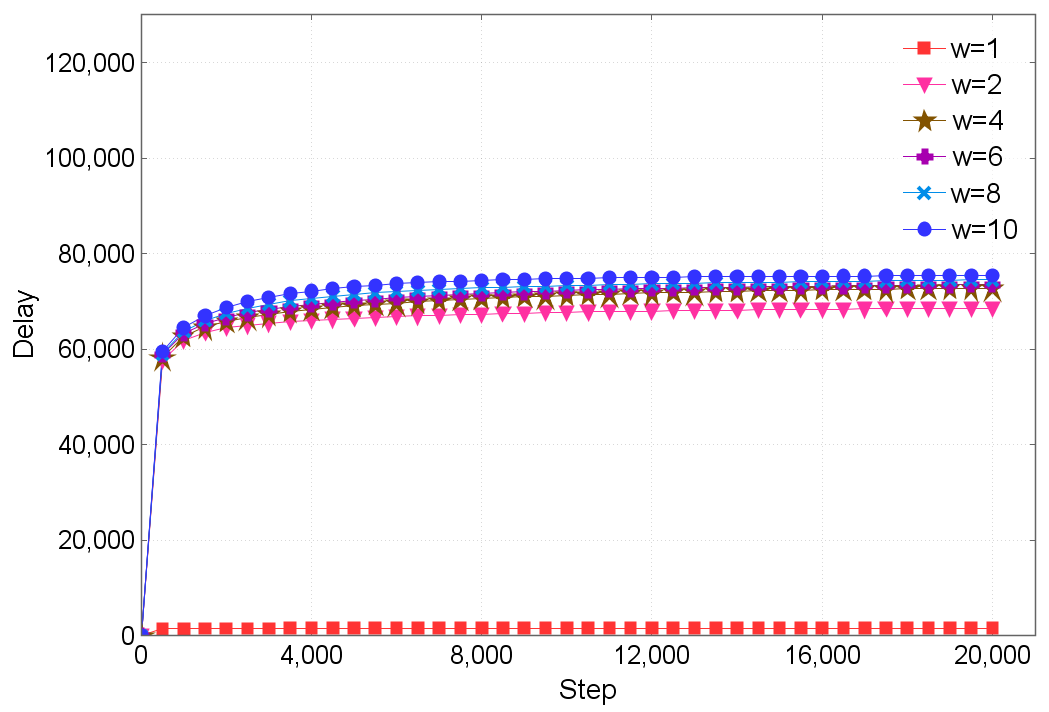
\includegraphics[width=.75\columnwidth]{delayPower}
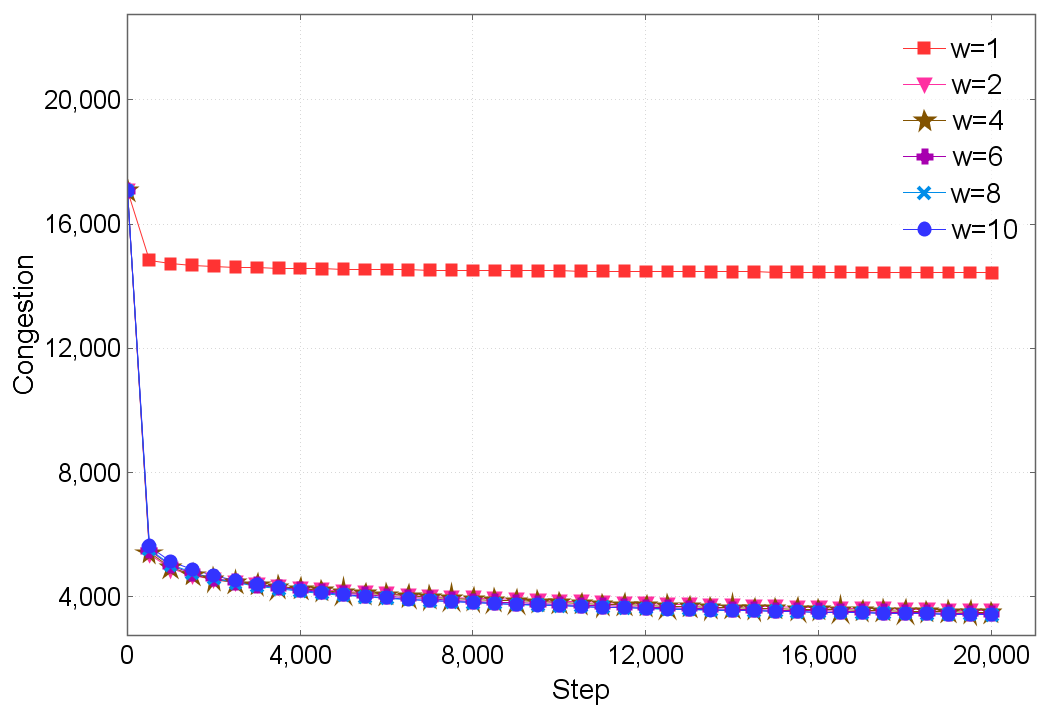
\includegraphics[width=.75\columnwidth]{congestionPower}
\caption{Delay and congestion with varying $w$, the weight on congestion. No matter the weight, the learning algorithm will not remove congestion while attempting to keep delay low. Additionally the cost to delay for when removing congestion is not a 1:1 mapping. A removal of 10,000 congestion adds 70,000 minutes of delay}
\label{delayCongestionPower}
\end{figure}

To solve this problem we introduce a greedy scheduler. The greedy scheduler converts sector congestion into a hard constraint, causing any amount of delay to achieve the goal. If any aircraft's flight plan violates the capacity constraint of any sector, it is forced to ground delay for 1 additional minute. Using the greedy scheduler forces congestion to become zero so that it does not need to be incorporated in the system utility.

Although the greedy scheduler is useful in removing congestion, it cannot also optimize delay. A simple solution would be to make every aircraft have a ground delay of 0, and have the greedy scheduler fix any conflicts, but this is highly suboptimal. Due to the congestion in the system, a delay of 0 for each aircraft would be suboptimal. The greedy scheduler assigns delay without taking into account agent coordination. An exhaustive search could then be used, but with such a large search space, this would be impossible. Reinforcement learning can discover a better assignment of ground delay for each aircraft, preventing the need to perform an exhaustive search. The previous cumulative delay calculation (Equation \ref{eq:Cumilative Delay}) can be used as the system-level reward for the new system.

\subsection{Hard Constraint Application}

Other approaches to solve the ATFMP have used only a small time window \cite{6095996}. We wanted to approach this problem with a full day of flight information, which is a 28-hour window (28 hours from the first takeoff in the day to the last landing aircraft that took off during the day). This increases the number of agents from a few thousand to 35,844. 

In this highly-congested coordination domain, it is difficult to achieve good performance without ensuring the agent's reward fully encapsulates the impact it had on the system, so we apply the difference reward. 

The difference reward was determined from the definition of the system-level reward (Equation \ref{eq:Cumilative Delay}):
%
\begin{equation}
D_i(z) = (-\delta(z)) - (-\delta(z-z_i + c_i)))\;,
\end{equation}
%
where \textit{$\delta(z)$} is the cumulative delay in the system and \textit{$\delta(z-z_j + c_j)$} is the cumulative delay of with agent $i$ replaced with counterfactual \textit{$c_i$}.

We combine the greedy scheduler with reinforcement learning, as shown in Figure \ref{LearningCycle}. All of the agents take an action, all actions are then modified using the greedy scheduler, and then each agent is assigned a reward based on the system after the greedy scheduler. Agents now receive a reward based on a modified version of the action they chose, leading to a noisy reward signal. Now agents have to simultaneously learn the right action to take and how their action becomes modified, complicating the learning problem \cite{journals/advcs/AgoginoT09}. Although the learning problem is now more complicated, congestion is removed from the systems, and agents still learn a well performing solution.

Combining the difference reward with the greedy scheduler causes a drastic increase in computation time. The difference reward requires an agent to be removed from the system, the greedy scheduler to reschedule all aircraft back into the system, and then compute the difference in delays. Rescheduling all 35,844 aircraft during each difference calculation makes this a computationally intractable solution. We use agent partitioning to greatly speed up the difference reward calculation by allowing the greedy scheduler to reschedule only the aircraft within the same partition as the removed agent, and reward agents only based on the delay of the other agents within their partition.

\begin{figure}[]
\centering
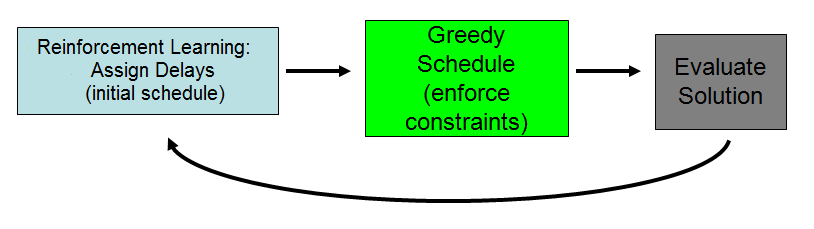
\includegraphics[width=1.0\columnwidth]{LearningCycle}
\caption{Evaluation using the greedy scheduler}
\label{LearningCycle}
\end{figure}

\subsection{Agent Partitioning}

The objective of agent partitioning is to leverage domain knowledge with the intention of partitioning together agents who impact each other. In this way we can treat each partition as its own independent problem, and solve them simultaneously.

Agent partitioning greatly helps the learning signal for the system-level reward, but not for difference reward. The key problem with the system-level reward is an agent receives too noisy of a learning signal to be able to learn a good policy. Partitioning assists the system-level reward by removing some of the noise caused by other agents, therefore creating a cleaner learning signal. On the other hand, the difference reward removes more noise from the learning signal than the agent partitioning, causing the difference reward to benefit less from the partitioning noise reduction, as seen in Section 4.1 and 4.2. The key benefit in combining agent partitioning and the difference reward is a large reduction in computation time. 

In many domains recomputing the reward may be costly. In the ATFMP computing the reward requires looping through all agents and computing the delay for all other agents. This becomes very computationally expensive when computing the difference reward, and requires agent partitioning to compute quickly.

%One way to circumvent this problem is function approximation of the domain using neural networks \cite{tumer-colby_gecco11}. In the work by Colby et. al, a neural network was used to predict wave energy converter power output with respect to key design variables. Although a function approximator can approximate the reward given simulator inputs, in largely complex domains with highly non-linear functions and a huge number of inputs (i.e. ATFMP), function approximation can be too costly, requiring millions of updates in order to accurately approximate a system.

One possible partitioning approach used by Agogino and Rios \cite{6095996} is to force every partition to be reward independent of every other partition. This requires a potential overlap of partitions, as typically many aircraft have partially or completely overlapping flight plans. Each partition is therefore a collection of overlapping flight plans with a small number of sectors unique to that partition. Although this approach achieves what we need, it typically results in $n$ partitions, where $n$ is the number of agents, and very large partitions due to overlapping flight plans. With around 35,000 aircraft this approach becomes prohibitively computationally expensive.

Instead of this approach, we applied Hierarchical Agglomerative Clustering (HAC) \cite{Agglomerative} to partition similar agents together. The similarity of each agent was computed as the number of similar sectors they had within their flight plan. In this way agents that impact each other are partitioned together. HAC was then applied using the average-linking metric and was saved at every iteration to obtain a varying size of partitions. Since our distance metric was a count of similar sectors, choosing the average-linking clustering metric was natural, as we are interested in how similar clusters are on average, rather than based on least or most similar members. This was accomplished all during the pre-processing of the flight plan data. Partitioning reduced the number of aircraft into a more manageable size for learning, from 35,844 to on the order of hundreds or thousands, depending on how long we run HAC.

When assigning a reward to an agent, only the delay of the agents within their partition is taken into account. Therefore, the greedy scheduler only needs to schedule the size of the partition during each difference reward calculation. This dramatically reduces the time complexity and allows the difference reward to be efficiently combined with the greedy scheduler. 

\section{Simulator Characteristics}
We present a multiagent approach to traffic flow management based on agents taking independent actions that maximize a system utility. All agents' actions are then simulated in a simple traffic flow management simulator. This simulator needs only to store sector and time information for each flight and compute congestion for each sector. From the simulation we can compute congestion and ground delay in the system and assign rewards to agents accordingly.

Due to the simplicity of our simulation requirements, using complicated simulators such as FACET \cite{FACET} and AgentFly \cite{Sislak:2008:AMA:1402744.1402755} would cause computation time problems. We chose to create our own flight simulator and scheduler because our simulation is simple; the only requirement is to keep track of sector capacities per time step, given a list of flight plans. Additionally, using reinforcement learning requires frequent sampling from data, meaning that using more advanced simulators would result in an unnecessarily large time complexity.

\section{Results}

In this section we test our approach in the ATFMP and compare learned policies under the difference reward and system-level reward to the strict greedy scheduling approach. Additionally, we take a look at the costs vs benefits of using agent partitioning in the ATFMP. We compare the time per learning step for each partition to the learned performance and discover the best partitioning for the problem setup. 

%\subsection{Learning with Soft Constraints}
%Agent partitioning allowed us to improve upon the learning approach with soft constraints. We tested the difference between using partitions and not using partitions and show here that using partitions dramatically improved performance for the system-level reward, but less for the difference reward.
%
%Agents within each partition are not always reward independent of all other agents. Making each partition reward independent would require no reward impact overlap among partitions, which is a difficult feat in this domain because many flight plans overlap each other for a small amount of time. Although difficult, making each partition reward independent is possible, but we found the partitioning consists of one very large partition, representing over 95\% of all aircraft, and many other smaller partitions. 
%
%When adding partitions to the original learning approach, some changes needed to be made to the congestion metric. Since agents are now given a reward based only on their small partition, the amount of time aircraft within a partition spend in a sector needs to be taken into account. If an aircraft only spends a few minutes in sector $i$, and a few hours in sector $j$, its impact on congestion in sector $j$ is much higher than sector $i$. We weighted the relative total congestion by the cumulative amount of time the aircraft within a partition are within a sector. The total congestion relative to partition $i$ is now a modified version of Equation \ref{eq:Global}, and becomes:
%
%\begin{equation}
%C_i(z) = \displaystyle\sum\limits_{s \in S} C_s(z)\;,
%\end{equation}
%
%where
%
%\begin{equation}
%C_s(z) = \displaystyle\sum\limits_{t \in T} \theta(C_{t,s} - S_s) (C_{t,s} - S_s) w_{i,s}\;,
%\end{equation}
%
%where $C_s$ is the capacity of sector $s$, $C_{t,s}$ is the capacity of sector $s$ at time step $t$, $S_s$ is the sector capacity of sector $s$, $\theta$ is a step function that equals 1 if its argument is greater than 0, and 0 otherwise, and $w_{i,s}$ is cumulative amount of time agents in partition $i$ are within sector $s$. The sum of the congestion over all sectors within a partition $i$'s flight plan make up the total congestion for partition $i$.
%
%\begin{figure}[]
%\centering
%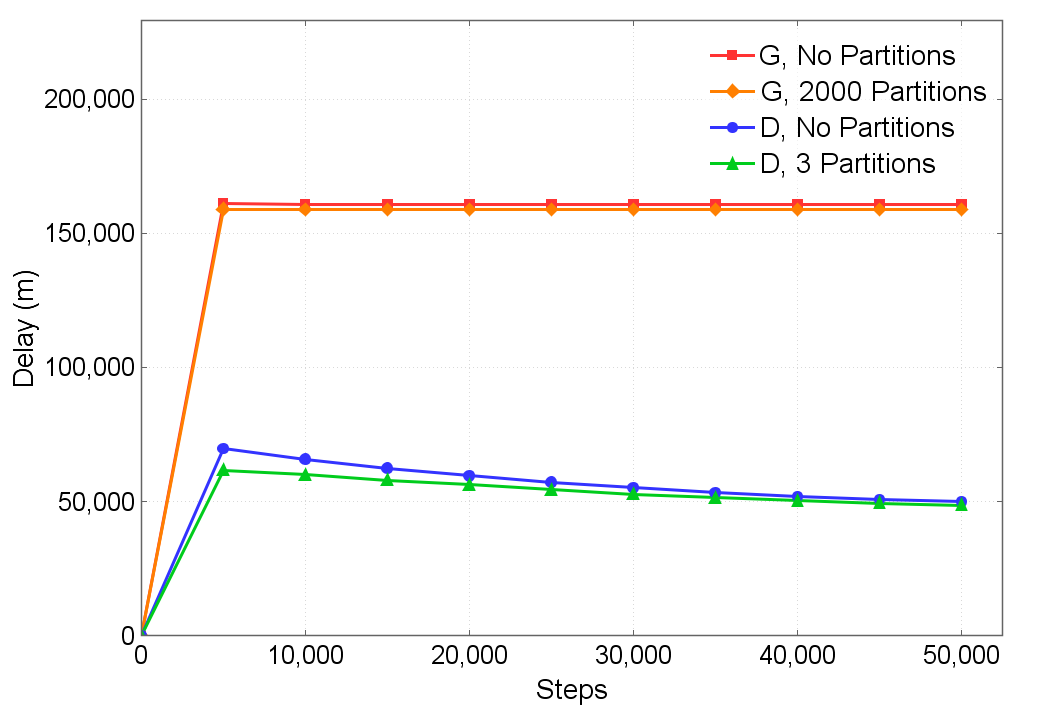
\includegraphics[width=.75\columnwidth]{ClusterVsNoClusterNonGreedy-Delay}
%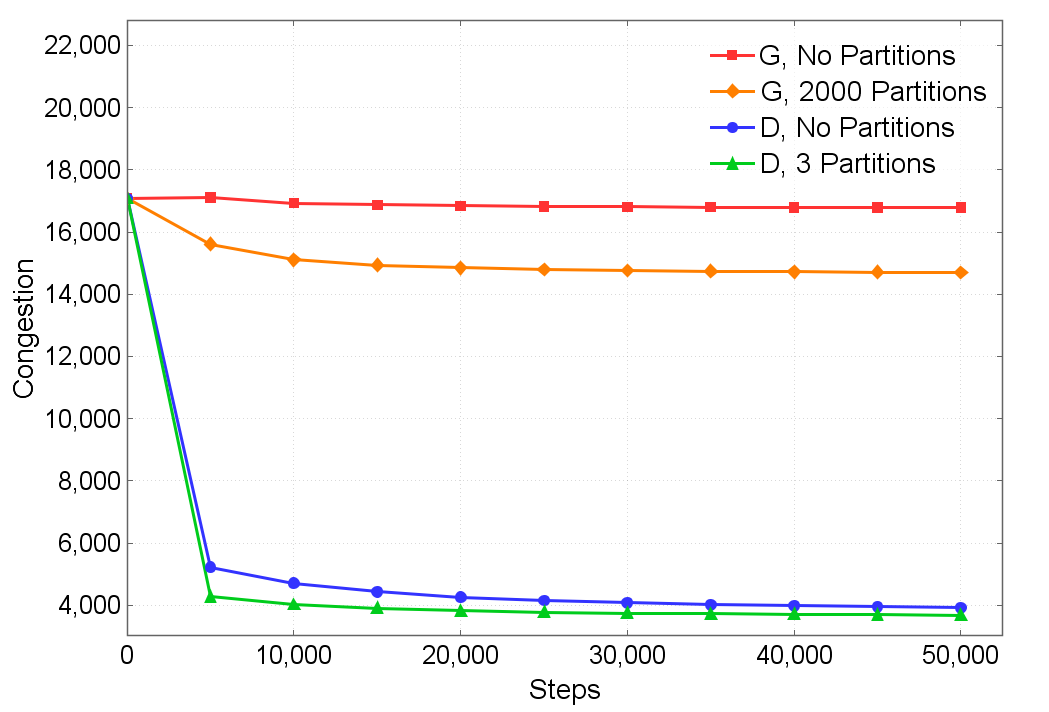
\includegraphics[width=.75\columnwidth]{ClusterVsNoClusterNonGreedy}
%\caption{Using the system-level performance as a reward does not work well in this large multiagent system. The difference reward was able to lower congestion much more, but could not manage to also reduce delay. Note that these are best performing experiments for the difference reward and system-level reward.}
%\label{NonClusterVsCluster}
%\end{figure}
%
%Figure \ref{NonClusterVsCluster} shows that the system-level reward performs better using partitions. The best partitioning performance was used, with a small number of partitions being used for the difference reward, and a large number of partitions used for the system-level reward. When looking closer at congestion and delay, we find that using the system-level reward does not improve delay at all, and only improves congestion slightly. There is too much noise caused by other agents within this system for the system-level reward to be a good evaluation. With the partitions, the noise is greatly reduced and therefore agents are given a better reward. The difference reward on the other hand is able to more easily capture an agents impact on congestion, and dramatically reduced congestion. The difference reward also benefits much less from the partitioning than the system-level reward. This is because the difference reward is able to reduce the signal-to-noise within the learning signal on its own, while the system-level reward requires the partitioning to attempt to accomplish the same noise reduction. The partitioning benefits the difference reward in time complexity, rather than performance.
%
%This is an acceptable solution if some congestion was allowed in the system, as both delay and congestion are greatly decreased. In our problem however, we would like to reduce congestion down to zero. This is only possible with the greedy scheduler.

\subsection{Learning with Hard Constraints}
By adding the greedy scheduler we were able to eliminate congestion by sacrificing delay. Some aircraft in normally highly-congested areas are forced to delay many hours, while most aircraft don't need to delay at all. Although high, this delay is required to guarantee a safe environment for all aircraft. 

This is a difficult scheduling problem that has a very specific solution. Although the greedy scheduler is suboptimal, it performs well in this domain without the use of agents. Most planes do not need to be delayed, and the ones that do can simply be delayed until no congestion occurs. This solution does not take into account any interactions between aircraft, and cannot perform the coordination required to reduce delay even further. Our approach finds a better solution by finding these subtle coordination situations and taking advantage of them.  

As mentioned earlier, the greedy scheduler gives a good, but not optimal scheduling policy. This leads us to use the greedy scheduling policy as a good place to start searching. Initializing each agent to choose zero delay reduces the overall amount of computation time needed to compute the difference reward by giving the agents a good policy from the start. Agents can then explore other actions with a frequency based on the exploration rate and can discover potentially better actions.
  
This greedy scheduler also includes bias when comparing experimental runs. The greedy scheduler schedules planes in order, resulting in different delay with a different ordering of aircraft. During partitioning, this ordering of aircraft changes for different partition sizes. Therefore, the initial greedy scheduling solution causes some bias in the trends we show here. For example, the greedy scheduler can initialize a particular partition to a better initial policy than a different partition size, causing bias in the comparisons. This greedy scheduling bias isn't large enough to impact the overall trend.

Figure \ref{ClusterRewardsGreedyG} shows that although using partitions are an improvement, using our system-level reward still does not minimize delay more than the simple greedy solution. This reward function does not give the agents an accurate enough learning signal to discover the subtle coordination improvements, and additionally takes a very long time to converge to a suboptimal solution. 

\begin{figure}[]
\centering
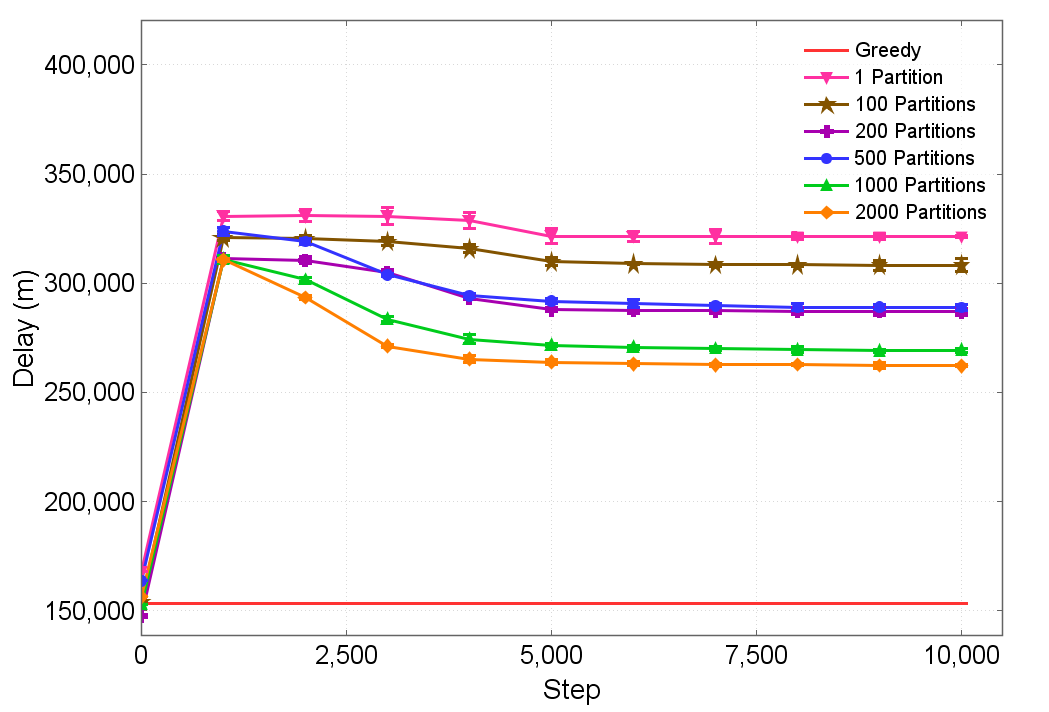
\includegraphics[width=1.0\columnwidth]{ClusterRewardsGreedyG}
\caption{The highest level of partitioning for the system-level reward (G) is displayed here and compared with zero partitioning and the greedy scheduler. The system-level reward performed worse with fewer partitions, but still better than zero partitioning. Even though partitioning performed better than zero partitioning, the system-level reward could not come close to beating the greedy scheduler. Using this learning approach, the system-level reward performance could never become better than the greedy scheduler.}
\label{ClusterRewardsGreedyG}
\end{figure}

The difference reward is able to communicate to the agents a reward that is more representative of their contribution to team performance. This reduced the the signal-to-noise ratio in the reward and greatly assists the agents in choosing the optimal action. This accurate reward allows agents to quickly find the subtle actions that will allow them to easily coordinate with other agents, thereby quickly reducing the delay more than the greedy scheduling solution. 

Figure \ref{ClusterRewardsGreedyG} and \ref{ATFMPOldDvsGreedy} shows the best-performing simulation using the system-level reward involved the highest number of partitions, while the best performing simulation using the difference reward used the lowest number of partitions. As the number of agents per partition increased, more agents affect the reward. The system-level reward has no way for an agent to filter out the noise of other agents, and therefore benefits more from a larger number of partitions. The difference reward on the other hand removes the noise out of the system-level reward and agents can therefore coordinate in the larger partitions easier.

\begin{figure}
\centering
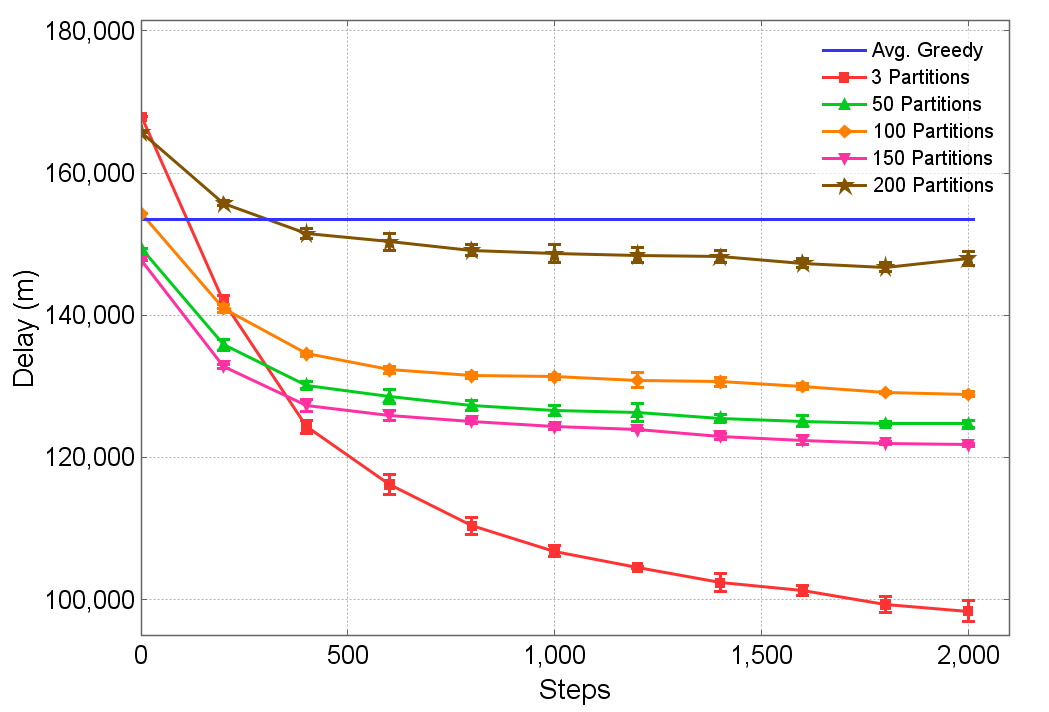
\includegraphics[width=1.0\columnwidth]{ATFMPOldDvsGreedy}
\caption{A closer look at the difference reward performance using the smaller number of partitions shows a 37\% improvement over the greedy scheduling solution.}
\label{ATFMPOldDvsGreedy}
\end{figure}

Although it would result in the best performance, using the difference reward with the greedy scheduler is an impossible task. With around 35,000 aircraft in the system, one reward step takes 3 hours due to the rescheduling needed at every difference calculation. Agent partitions allowed us to greatly decrease simulation time, as only agents within a partition need to be rescheduled during the difference calculation. Graph \ref{ATFMPOldDvsGreedy} shows the magnitude of performance gain when using the difference reward and partitioning, while Table \ref{ATFMPOldTable} shows that the speedup of using different partition sizes is significant, but has a high cost to performance. Since partitions had some overlap, actions in one partition may affect the agents in another partition, meaning that the higher the number of partitions the less information the agents receive of the environment. A smaller number of partitions end up leading to better overall performance at the cost of computation time.

\subsection{Partition Comparison for Hard Constraints}
Speed and performance of partitions were negatively correlated. As the number of partitions reduced, the greedy scheduler was required to schedule more planes per difference calculation. This greatly increased the amount of time per learning step. Additionally, with a smaller number of partitions, planes that slightly affected each other were partitioned together. This allowed higher quality learning since an agent's reward encompassed the effects of at most all of the other agents that impact it. 

This speed and performance correlation also occurs within the same partition. As the delay decreases, more agents switch from taking the zero delay action to taking a more intelligent action allowing better scheduling. This means that the agent no longer equals the counterfactual, and the difference reward calculation cannot be skipped. Table \ref{ATFMPOldTable} shows this in more detail. This table compares the amount of time taken per simulation step to the final performance.

\begin{table}
\begin{tabular}{|l|c|c|}
\hline
& Average Time per &Converged Performance\\
Partitions & Learning Step (s) &Delay (m)\\
\hline
Greedy & * & 153502 \\
\hline
3 & 483.76 & 97688 \\
\hline
50 & 42.11 & 124056 \\
\hline
100 & 22.43 & 128021 \\
\hline
150 & 20.91 & 121074 \\
\hline
200 & 17.37 & 145844\\
\hline
250 & 14.27 & 152402 \\
\hline
\end{tabular}
\caption{With the greater number of partitions, the learning performance decreases and speed increases. Note that the outlier is a artifact of the greedy scheduler discussed in this section.}
\label{ATFMPOldTable}
\end{table}

The agent partitioning allows applications to become very situation dependent. If results need to be found very quickly, a larger number of partitions could be used, and this approach will find a policy still better than using the greedy scheduler. On the other hand if time spent is not important, the smaller number of partitions will result in a very good policy 37\% better than the greedy scheduler, and still 450x faster per learning step than non partitioning based approaches. The same trends found in this section are expected in the partitioning using RUBI.


\section{Conclusion}

The ATFMP method introduced is based on agents representing airport gates within the NAS choosing aircraft ground delay with the intent of minimizing delay within the system. It uses reinforcement learning in combination with the difference reward and hard constraints on congestion. This is typically an impossible problem, but we introduce agent partitions to dramatically reduce the time complexity by  450x per simulation step with a 37\% increase in performance over the greedy solution. The different sizes of partitions also allowed the implementation to vary with the situation. If results need to be computed quickly, a large number of partitions could be used, where a smaller number of partitions could be used if performance was more important than speed. In this case a solution could reduce the time complexity by 5400x per learning step, with a 20\% increase in performance over the greedy solution. The ease of adding simple ground delays in combination with the large increase in performance over currently used approaches makes this approach easily deployable and effective.

\label{sec:CONCLUSION}


\bibliographystyle{plain}
\bibliography{thesis}

\end{document}
